\chapter{User Guide}

This appendix walks through everything you need to get the framework running - from cloning the repository to training your own models and evaluating them against Stockfish. All commands assume you're working from the \textbf{root} of the project directory. Running scripts from within a subdirectory will break relative path resolution and cause import errors, so don't do it.

\section{Setup and Installation}

The quickest way to get started is with the provided setup script, which creates a virtual environment and installs all dependencies in one step:

\begin{verbatim}
./setup.sh
source .venv/bin/activate
\end{verbatim}

If you'd rather do it manually:

\begin{verbatim}
python3 -m venv .venv
source .venv/bin/activate
pip install -e ".[dev]"
\end{verbatim}

The framework auto-detects your hardware at startup and selects the best available backend - CUDA if you have a compatible NVIDIA GPU, MPS on Apple Silicon, or CPU as a fallback. You don't need to configure this yourself.

\section{Downloading Pre-Trained Checkpoints}

Training from scratch takes days on GPU. If you just want to run evaluations, download the pre-trained checkpoints directly:

\begin{verbatim}
python3 scripts/download_models.sh
\end{verbatim}

This populates \texttt{runs/models/} with checkpoints for all six architectures. The Lichess puzzle dataset and the pre-processed training parquet files are available separately on Kaggle at \texttt{https://www.kaggle.com/datasets/bhavyasingh2611/\\lichess-evals-stripped}, if you want to retrain from the same data.

\section{Training Models}

Training a model is a single command. The recommended way is to use the pre-written shell scripts in \texttt{scripts/training/}, which encode the exact hyperparameter schedules used in the experiments:

\begin{verbatim}
./scripts/training/resnet_train.sh
\end{verbatim}

Or, if you want to run a quick custom training run:

\begin{verbatim}
python scripts/train.py --model resnet --epochs 20 --name my_run
\end{verbatim}

Supported backbone values are: \texttt{convnet}, \texttt{resnet}, \texttt{square\_transformer}, \texttt{piece\_transformer}, \texttt{gcn}, and \texttt{gat}. Checkpoints, metrics, and logs are written to \texttt{runs/<name>/training/<model>/}.

\section{Benchmarking Against Stockfish}

Once you have a checkpoint - either downloaded or trained - you can evaluate it against Stockfish. Again, the simplest path is the pre-written benchmark scripts:

\begin{verbatim}
./scripts/benchmark/resnet_benchmark.sh
\end{verbatim}

Or manually, pointing at a specific checkpoint:

\begin{verbatim}
python scripts/benchmark.py --model resnet \
    --checkpoint runs/models/resnet/resnet_100M_e15.pt
\end{verbatim}

Each benchmark run generates PGN files with embedded Stockfish evaluations (viewable in Lichess, Chess.com, or ChessBase), along with a summary report. Results land in \texttt{runs/<name>/benchmark/}.

\section{Puzzle Benchmarking}

For a faster, more targeted evaluation, the puzzle benchmark assesses tactical accuracy on stratified Lichess puzzles and produces an estimated Elo rating:

\begin{verbatim}
./scripts/puzzle_benchmark/resnet_puzzle_benchmark.sh
\end{verbatim}

Or manually:

\begin{verbatim}
python scripts/puzzle_benchmark.py --backbone resnet \
    --weights runs/models/resnet/resnet_100M_e15.pt
\end{verbatim}

Puzzle data lives in \texttt{data/puzzles/}. The stratified sampling ensures the difficulty distribution matches real Lichess ratings, so the Elo estimate is reasonably calibrated.

\section{Configuration}

All hyperparameters live in \texttt{config/settings.yaml}. The key sections are:

\begin{itemize}
    \item \textbf{Model}: backbone type, head type (\texttt{policy}, \texttt{value}, or \texttt{dual}), layer counts, embedding dimensions.
    \item \textbf{Training}: batch size, learning rate, weight decay, LR scheduler, gradient clipping.
    \item \textbf{Hardware}: device selection, data loader worker count.
\end{itemize}

Individual settings can be overridden with CLI flags without editing the file, which makes it easy to run quick ablations. That said, the YAML snapshot is what gets saved alongside each checkpoint - so if you want a run to be fully reproducible, don't rely on CLI overrides alone; make a copy of the config file first.

\begin{figure}[htbp]
    \centering
    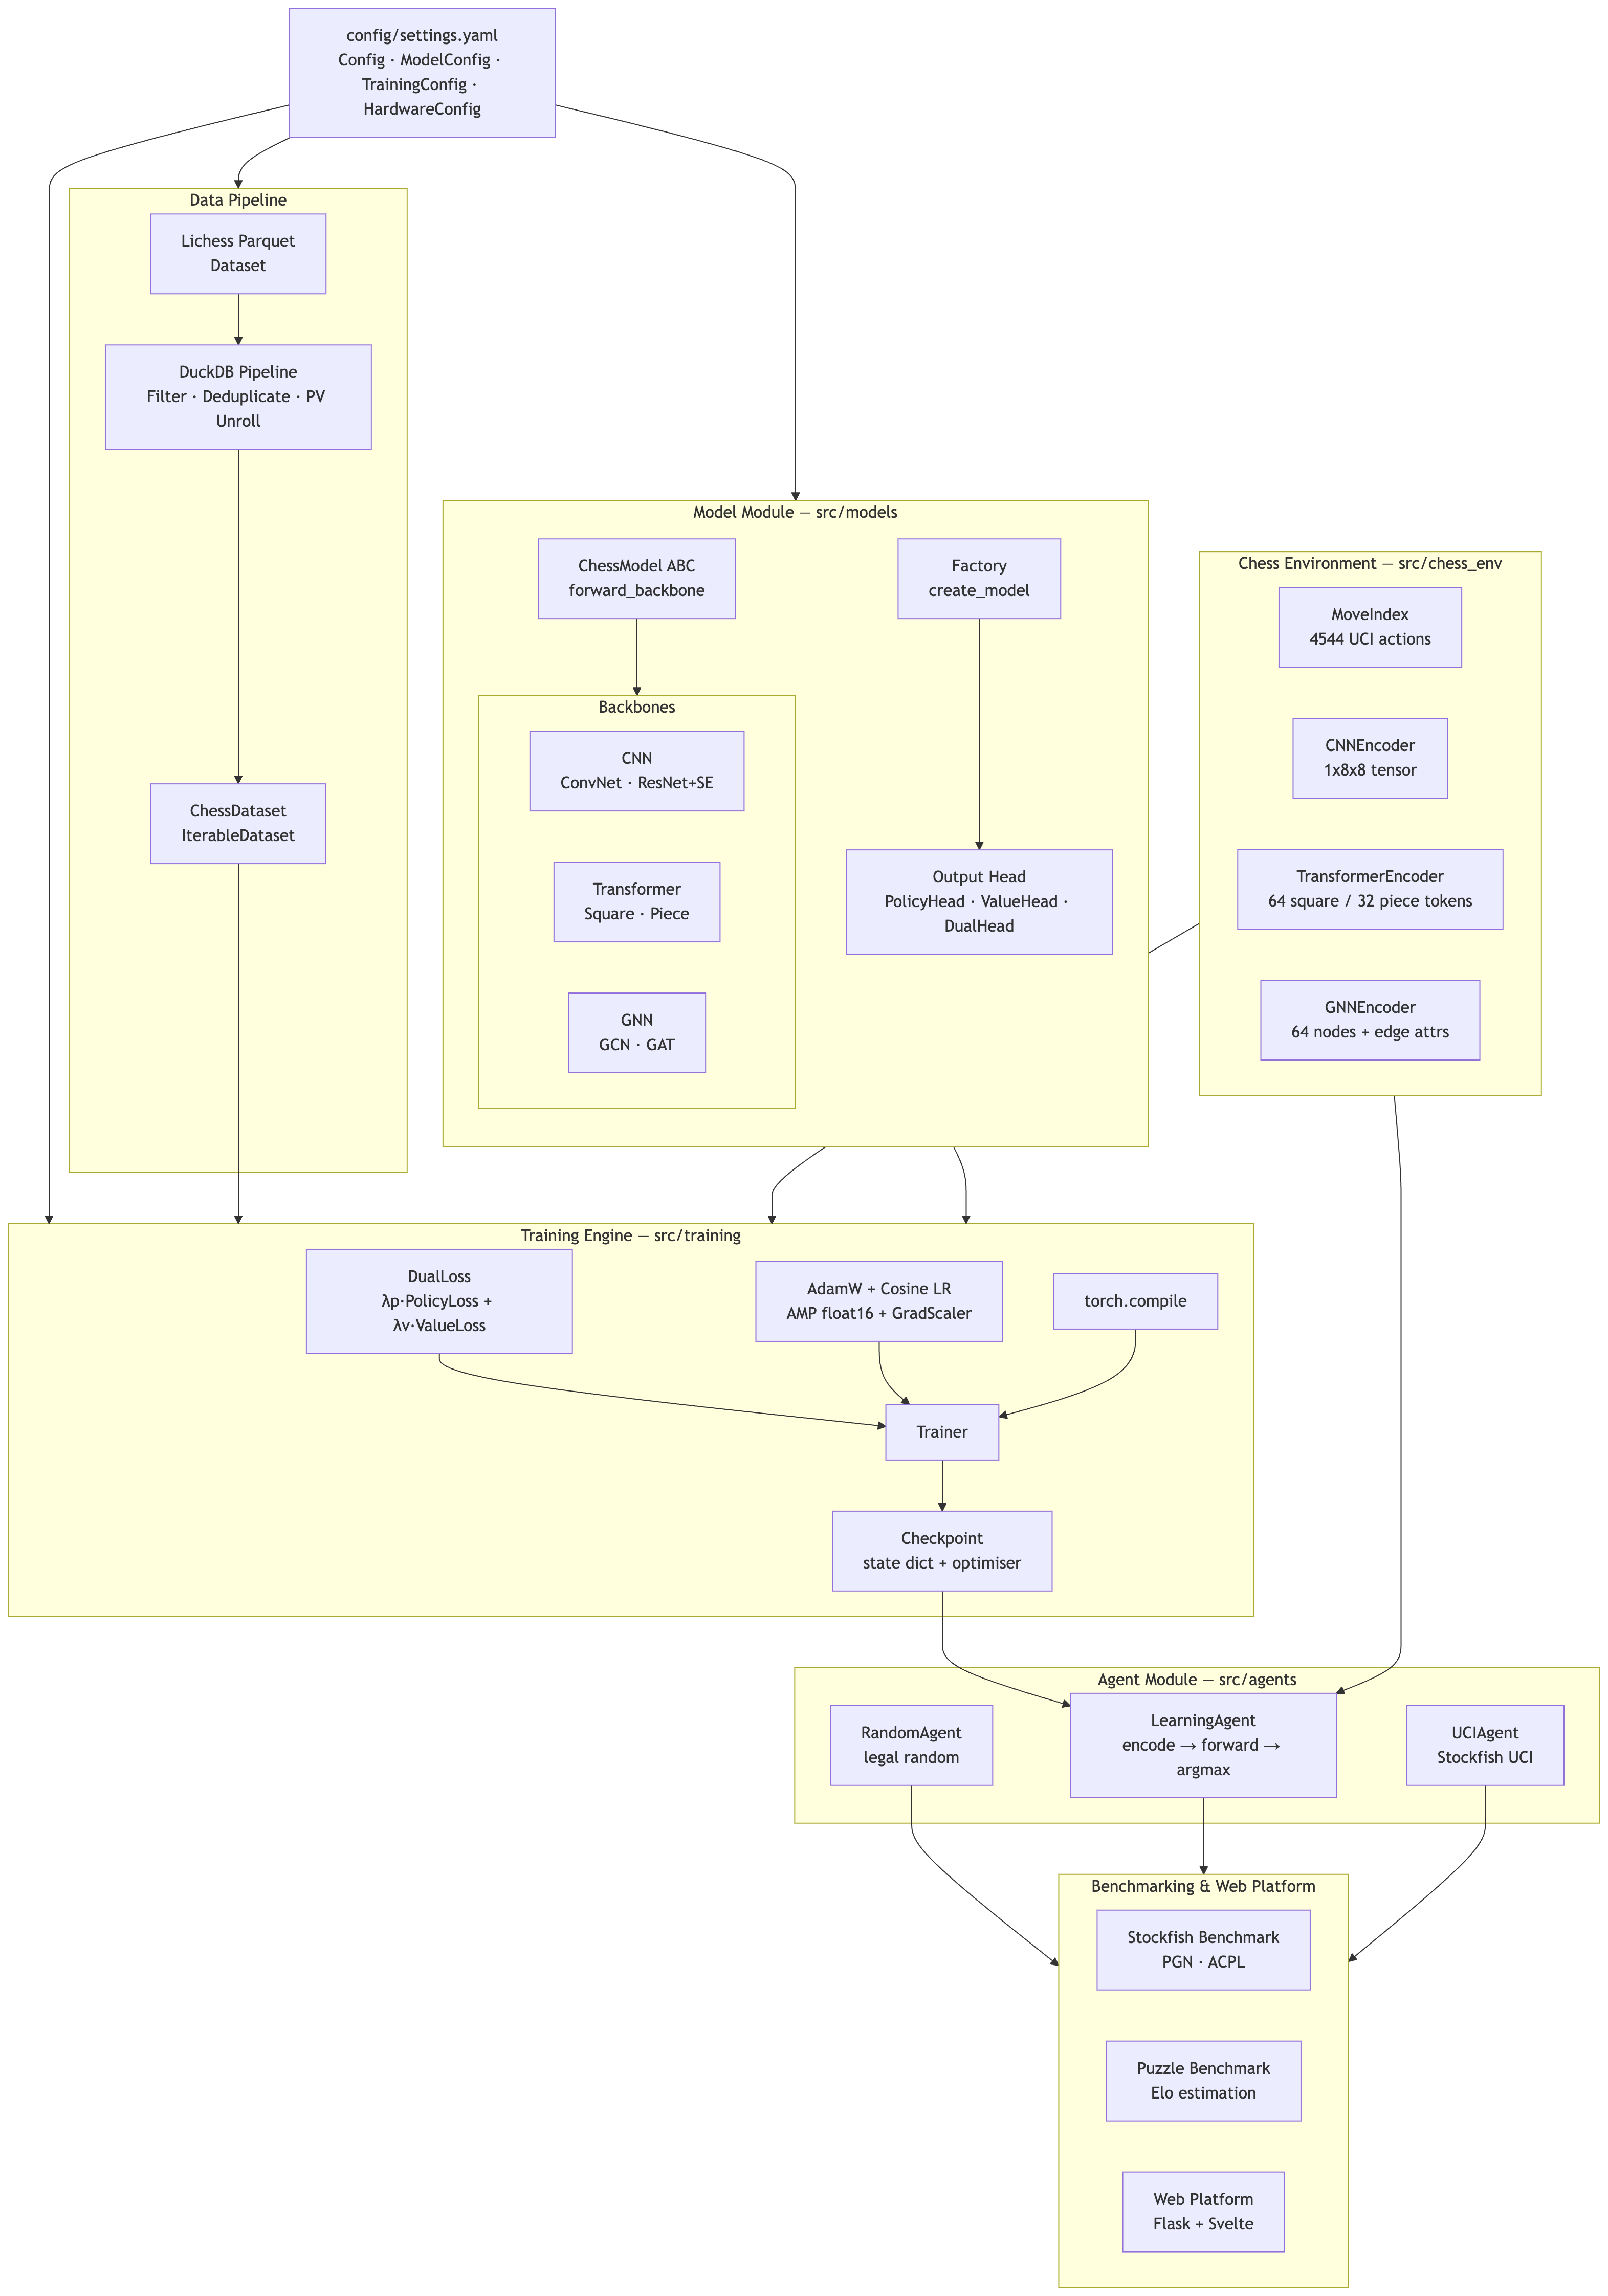
\includegraphics[width=0.9\linewidth]{figures/flow.png}
    \caption{End-to-end module flow, from raw Lichess data through training to benchmarking and the web platform.}
    \label{fig:framework_module_flow}
\end{figure}
